\section{Methodology}
\subsection{Iterative and Incremental Model}

For the successful execution of this project, the Iterative and Incremental Development Model has been adopted. This model is particularly well-suited for projects involving machine learning and deep learning, where experimentation, continuous refinement, and frequent testing are essential. In this approach, the system is built gradually through repeated cycles (iterations), where each cycle results in a functional version of the system. This allows for early evaluation of the model's performance and provides opportunities to identify and correct issues, such as data imbalance or underfitting, in earlier stages. Each iteration adds new features or improvements while preserving the core functionality developed in previous cycles.

The iterative model is especially beneficial for deep learning projects like brain tumor detection and classification, where model architecture, data preprocessing techniques, and hyperparameters often require multiple rounds of testing and fine-tuning. It enables the team to begin with a basic \gls{cnn} implementation and progressively improve the system by integrating advanced techniques such as transfer learning using \gls{vgg16}. Moreover, this model promotes adaptability, allowing changes in design based on validation feedback and model accuracy. It also facilitates parallel development of modules such as data preparation, model training, evaluation, and documentation, ensuring steady progress and reducing overall project risk.
\begin{figure}[h]
    \centering
    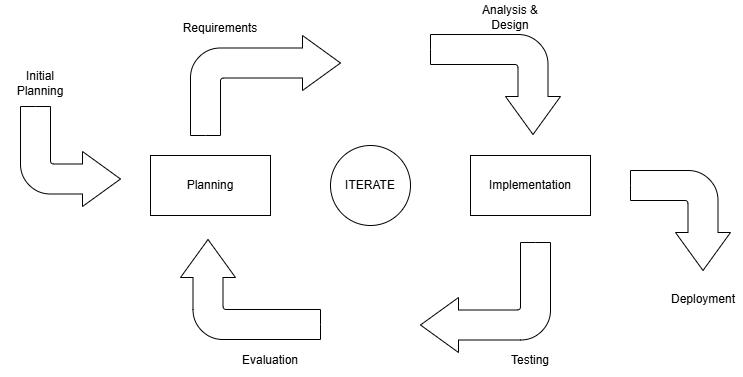
\includegraphics[width=1\linewidth]{Images/model.png}
    \caption{Iterative and Incremental model}
    \label{fig:enter-label}
\end{figure}

\subsection{Requirement identification}
\subsubsection{Development Requirements}

\begin{table}[h!]
\centering
\caption{Development System Specifications}
\begin{tabularx}{\textwidth}{@{} l X @{}}
\toprule
\textbf{Component} & \textbf{Specification} \\
\midrule
Processor (CPU) & Intel i5 (8th Gen or newer) / AMD Ryzen 5 \\
GPU & NVIDIA GTX 1050 Ti (4 GB VRAM, CUDA support) \\
RAM & 8 GB \\
Storage & 100 GB SSD \\
Operating System & Windows 10 / Ubuntu 20.04 \\
Programming Language & Python 3.8+ \\
Libraries/Frameworks & TensorFlow / Keras, Pillow, NumPy, Matplotlib \\
IDE / Tools & VS Code / Jupyter Notebook / Google Colab \\
\bottomrule
\end{tabularx}
\end{table}

\subsubsection{Deployment Requirements}

\begin{table}[h!]
\centering
\caption{Deployment System Specifications}
\begin{tabularx}{\textwidth}{@{} l X @{}}
\toprule
\textbf{Component} & \textbf{Specification} \\
\midrule
Hosting Platform & Local Server / AWS EC2 \\
CPU & Intel i3 or equivalent \\
RAM & 4 GB \\
Storage & 20 GB SSD \\
GPU & Not required (for inference-only deployment) \\
Operating System & Windows/Linux-based VM or container \\
Web Framework & Flask / Streamlit \\
Deployment Tools & Docker (optional), Git, Nginx (optional for production) \\
\bottomrule
\end{tabularx}
\end{table}

% \begin{figure}[h]
%     \centering
%     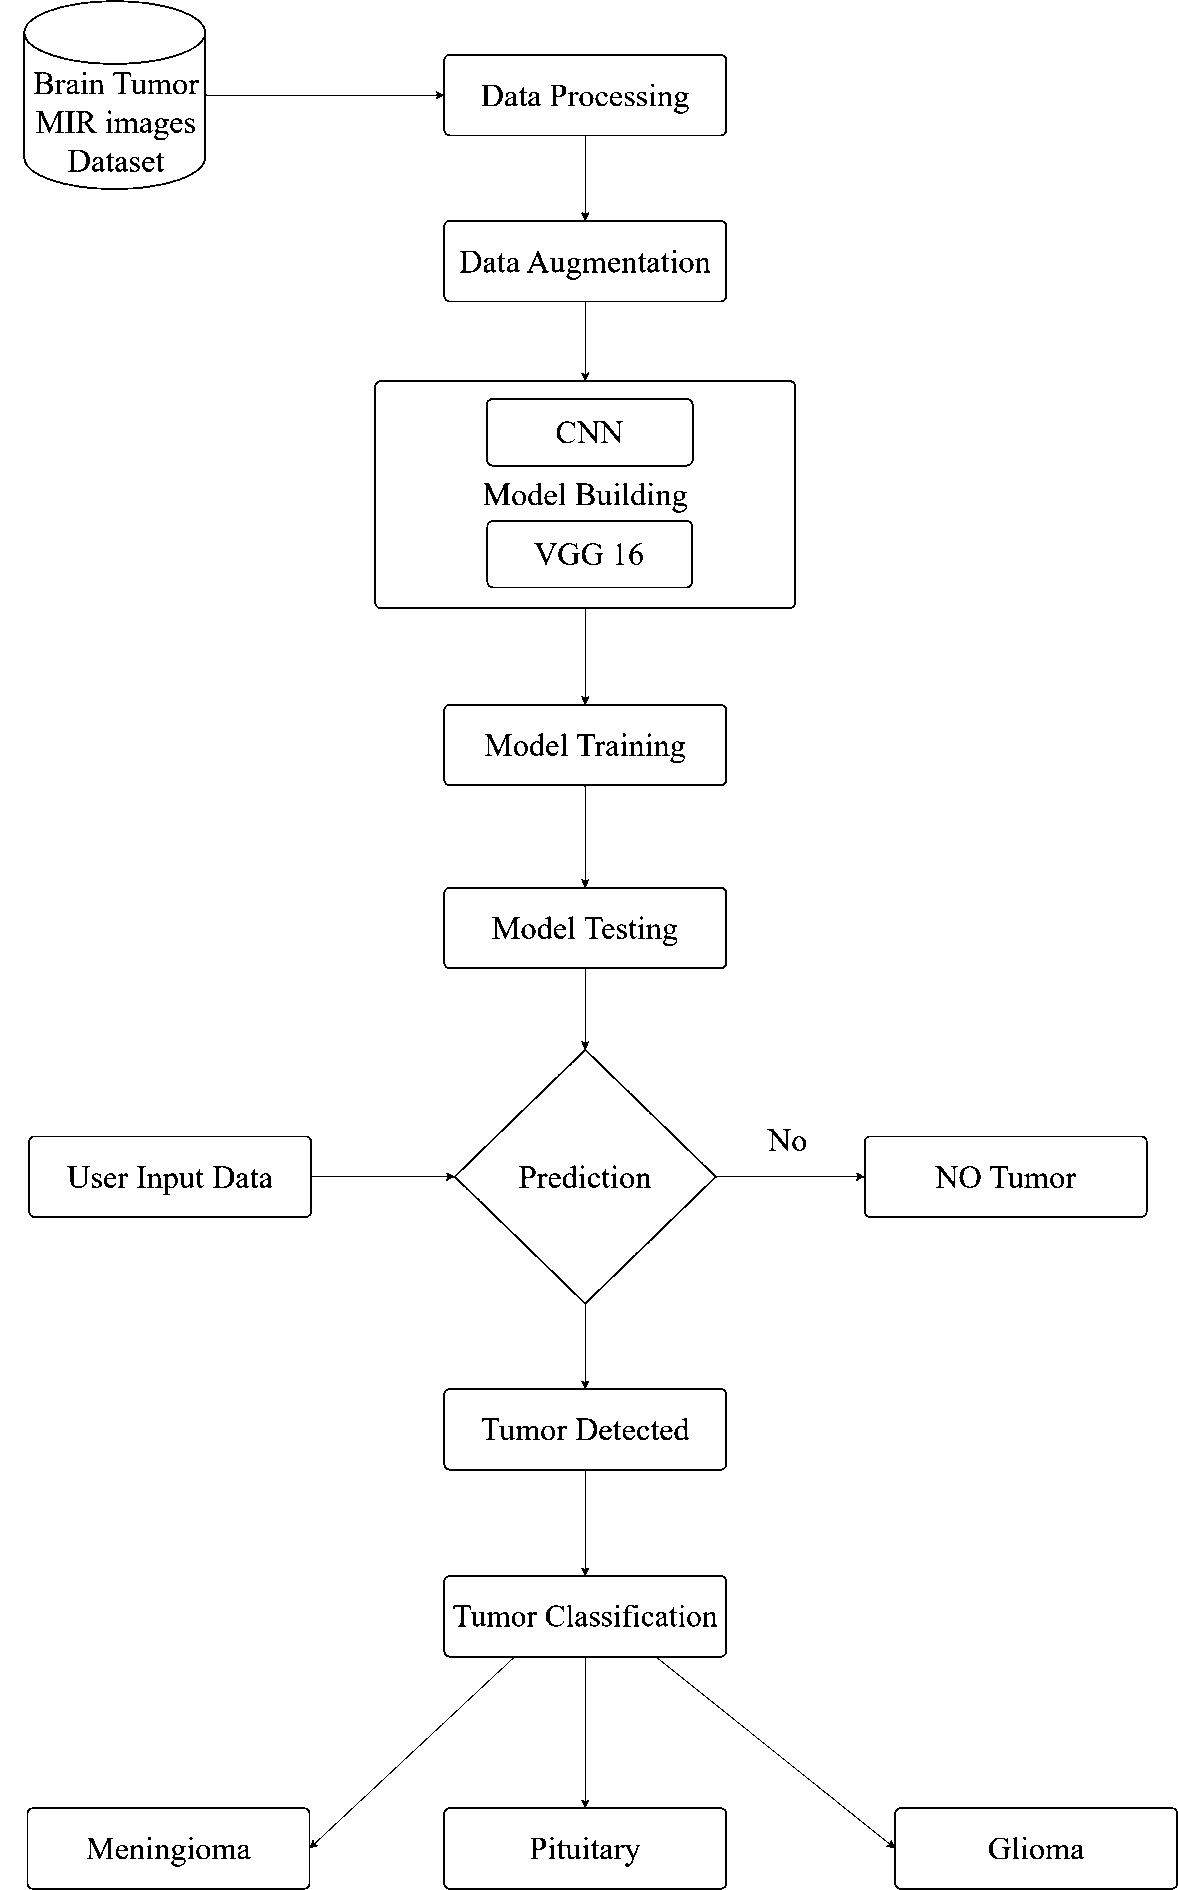
\includegraphics[width=0.5\linewidth]{Images/flow.png}
%     \caption{Caption}
%     \label{fig:enter-label}
% \end{figure}
% Discuss how previous work relates to your project and identify any limitations or gaps that your project aims to address.

\subsubsection{Study of Existing System / Literature Review}
Convolutional Neural Networks (CNNs) have significantly advanced the field of medical image analysis, particularly in brain tumor classification from MRI scans. These models automatically extract spatial hierarchies of features from pixel data, eliminating the need for manual feature engineering. Transfer learning, especially using architectures like VGG16 pretrained on ImageNet, has been widely adopted due to limited labeled medical datasets. While some studies report classification accuracies exceeding 97\% using fine-tuned VGG16 models \cite{mathivanan2024} \cite{babu2023} \cite{khaliki2024}, several others have encountered challenges in achieving such high accuracy due to dataset limitations, overfitting, and task complexity.

For instance, Zohra et al. (2024) compared a custom CNN and a VGG16-based model on a small, imbalanced brain MRI dataset and reported test accuracies of only 72\% and 75\%, respectively. The authors attributed this to the small dataset size and class imbalance, which led to overfitting and poor generalization, even though the training accuracy exceeded 98\% \cite{zohra2024}. Similarly, Srinivasan et al. (2024) proposed a hybrid deep CNN for five-class brain tumor classification, achieving an overall test accuracy of 93.81\%, with the lowest per-class accuracy of 95.6\% for pituitary tumors. The increased difficulty of multi-class classification and the limited number of training samples for some tumor types were cited as contributing factors \cite{srinivasan2024}.

Aksoy (2025) also employed a VGG16-based transfer learning approach on a binary classification task using a private MRI dataset of 7,000 images. While the model achieved perfect training accuracy, the validation accuracy plateaued at 94\%, and the test accuracy remained slightly below 95\%, highlighting issues with overfitting and potential limitations of transfer learning in handling medical images \cite{aksoy2025}. These findings demonstrate that while CNNs and VGG16 offer powerful tools for tumor analysis, achieving state-of-the-art performance consistently requires robust datasets, proper augmentation, and careful tuning of model architectures.

\subsubsection{Requirement Analysis}
\subsection{Feasibility Study}
\subsubsection{Technical}
 The technical feasibility of this project is strong, as it builds on existing, well-documented deep learning architectures particularly Convolutional Neural Networks (\gls{cnn}s) and pre-trained models like \gls{vgg16}. Platforms such as TensorFlow and PyTorch offer robust tools for training and deploying neural networks, while GPU-enabled environments like Google Colab or local setups with mid-range NVIDIA GPUs support high-performance computing without the need for expensive hardware. Furthermore, publicly available \gls{mri} datasets (e.g., Keggle) provide high-quality, labeled images necessary for model development and evaluation. Given these readily available tools and datasets, implementing and fine-tuning a \gls{cnn} model using transfer learning is technically viable.
 
\subsubsection{Operational}
From an operational standpoint, the system is intended to assist medical practitioners or researchers in detecting and classifying brain tumors (such as glioma, meningioma, and pituitary tumors) from \gls{mri} images. The proposed system can be developed as a standalone diagnostic tool or integrated into a web-based interface for ease of use. This project can be executed by a small development team with basic knowledge in Python programming, image processing, and machine learning. With clear deliverables in model training, performance evaluation, and a basic front-end deployment the system can be developed within the given academic timeline and available manpower.

\subsubsection{Economic}
Economically, the project is viable for an academic institution or student-level research. Development can be carried out using free and open-source tools, including Python, Jupyter Notebook, TensorFlow, Keras, and Google Colab (for cloud-based training). No expensive commercial licenses are required. If a more powerful hardware setup is desired, services like Kaggle Kernels or Google Cloud's free tier may be used. Thus, the overall cost of development remains minimal, making the project economically sustainable.

% \begin{table}[h]
%     \centering
%     \caption{sample Cost-Benefit Analysis of the Proposed Project}
%     \begin{tabular}{@{}llcc@{}}
%         \toprule
%         \textbf{Item} & \textbf{Description} & \textbf{Cost (\$)} & \textbf{Benefit (\$)} \\ \midrule
%         Development Costs & Software Development & 15,000 & - \\
%         Hardware Costs & Servers and Equipment & 5,000 & - \\
%         Training Costs & User Training Sessions & 2,000 & - \\
%         Maintenance Costs & Annual Maintenance & 1,000 & - \\
%         \midrule
%         \textbf{Total Costs} &  & \textbf{23,000} & - \\ \midrule
%         Increased Efficiency & Time Savings & - & 30,000 \\
%         Improved User Satisfaction & User Feedback & - & 10,000 \\
%         Revenue Increase & New Customers & - & 20,000 \\
%         \midrule
%         \textbf{Total Benefits} &  & - & \textbf{60,000} \\ \midrule
%         \textbf{Net Benefit} &  & \textbf{23,000} & \textbf{37,000} \\ 
%         \bottomrule
%     \end{tabular}
%     \label{tab:cost-benefit}
% \end{table}

 Analyze the cost-effectiveness of the project. Consider the budget, expected benefits, and potential return on investment. Provide a cost-benefit analysis to justify the project's financial viability.
 
\subsubsection{Schedule(Gantt chart showing the project timeline)}
\begin{figure}[H]
    \centering
    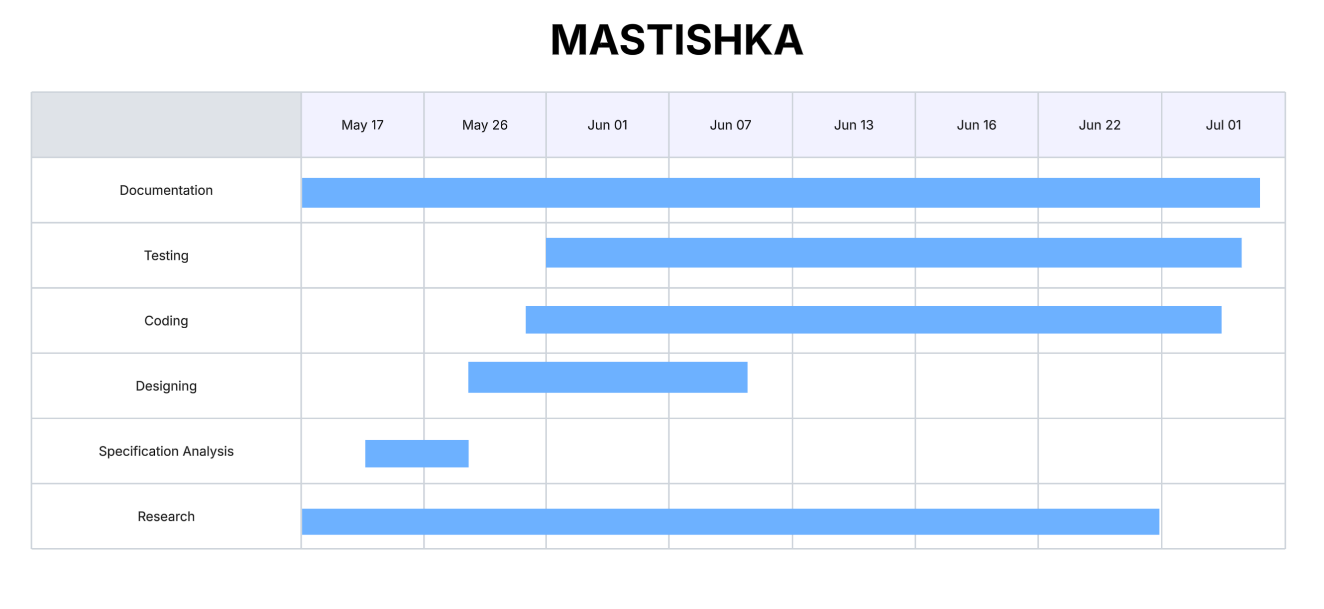
\includegraphics[width=1\linewidth]{Images/gantt.png}
    \caption{Sample Gantt Chart demonstrating schedule feasibility}
    \label{fig:enter-label}
\end{figure}
  
\subsection{High-Level Design of System}
\subsubsection{Methodology of the proposed system}
\textbf{Dataset Overview}

The project utilizes publicly available \gls{mri} brain tumor datasets provided on platform called Keggle (https://www.kaggle.com/datasets/masoudnickparvar/brain-tumor-\gls{mri}-dataset) and the Brain Tumor Segmentation (BraTS) challenge datasets. These datasets contain 7023 of \gls{mri} images categorized into different tumor types—typically glioma, meningioma, pituitary tumor, and no tumor. The images are generally grayscale, in JPG format, and vary in dimension (commonly 240×240 or 512×512 pixels). Each image is labeled according to its tumor class, making the dataset suitable for supervised learning. The datasets often contain minor class imbalance, which must be addressed in the preprocessing and balancing phase.

\textbf{Data Pre-processing and Feature Extraction}

\gls{mri} images often contain noise, inconsistent brightness, and irrelevant background structures like the skull, which can negatively impact model performance. Therefore, pre-processing is an essential step. The following transformations are applied:
    \begin{enumerate}[label=\roman*.]
    \item Data augmentation techniques such as random rotations, zooming, flipping, and shifting are applied to artificially expand the dataset and improve model generalization.
    \item Grayscale normalization or conversion to 3-channel format for compatibility with pre-trained models.
    \item Noise is eliminated using morphological operations, specifically a combination of erosion and dilation.
    \item Skull-stripping (if not already applied in the dataset) to isolate brain tissue.
    \item Resizing all images to a consistent dimension (e.g., 224×224 pixels, 240×240 pixels) to match the input size required by \gls{vgg16} and \gls{cnn} respectively.
\end{enumerate}
In terms of feature extraction, the \gls{vgg16} model, pre-trained on ImageNet, is used as a feature extractor. Its initial layers are retained to utilize its learned low-level features (edges, shapes), while the final classification layers are replaced and fine-tuned on the brain \gls{mri} data.

\textbf{Data Visualization and Balancing Dataset}

To begin understanding the dataset, we performed exploratory data visualization. The distribution of images across different classes was analyzed using bar charts, and random samples of \gls{mri} scans were displayed to visually inspect class characteristics.

Visualization played a critical role in identifying potential class imbalance. Our dataset, which includes labeled \gls{mri} images indicating tumor or no-tumor presence, showed some skewed class distributions. To mitigate bias during training, we used the ImageDataGenerator class with balanced sampling by setting class\_mode='categorical' and shuffle=True, helping ensure that batches were representative of both classes.

While explicit over-sampling or under-sampling techniques such as SMOTE or resampling were not used, the impact of minor imbalance was reduced via image augmentation and balanced batch generation during training.

\textbf{Data Splitting}

The dataset was partitioned into training and validation subsets using TensorFlow’s `ImageDataGenerator` with a validation split of 20\%. This split ensures that the model's performance is evaluated on unseen data during training. The training generator was configured with real-time data augmentation—applying random rotations, zooming, shearing, and flipping to prevent overfitting and improve generalization.

\begin{itemize}
    \item \textbf{Training Set:} 80\% of the data, augmented and shuffled.
    \item \textbf{Validation Set:} 20\% of the data, used for monitoring model performance.
\end{itemize}

\textbf{Model Testing}

After training, both the custom \gls{cnn} and \gls{vgg16}-based models were evaluated on a separate test set to assess real-world performance. Predictions were generated, and the results were compared against ground truth labels using the following metrics:

\begin{itemize}
    \item \textbf{Accuracy:} The ratio of correctly predicted images.
    \item \textbf{Confusion Matrix:} Used to analyze true positives, false positives, true negatives, and false negatives.
    \item \textbf{Classification Report:} Provides precision, recall, and F1-score for each class.
\end{itemize}

These metrics provided a holistic view of model performance and revealed strengths and weaknesses in classifying tumor vs. non-tumor \gls{mri} scans. Visualization of the confusion matrix and sample predictions helped interpret model behavior and supported further refinement.

\subsubsection{Flow Chart}
\begin{figure}[H]
    \centering
    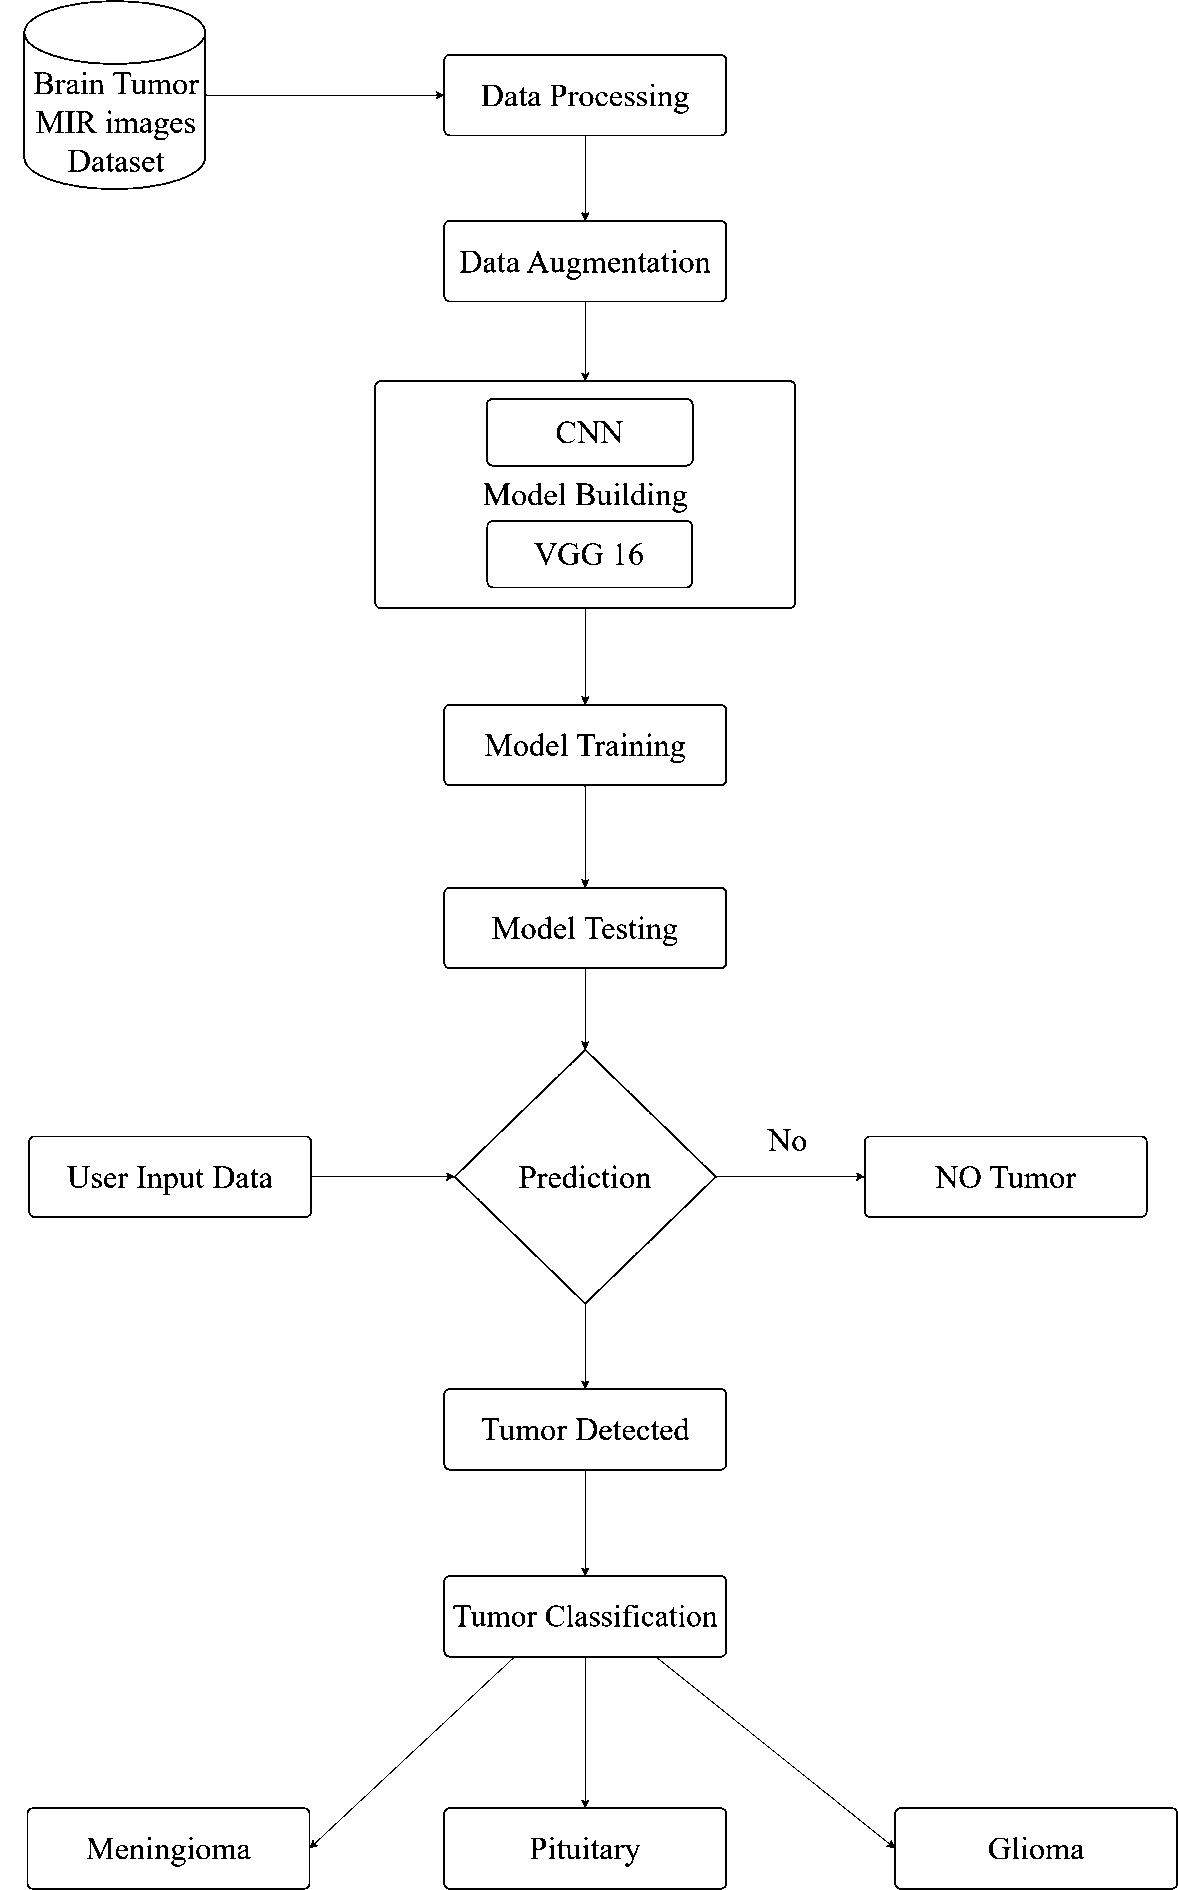
\includegraphics[width=0.85\linewidth]{Images/flow.png}
    \caption{Working Mechanism}
    \label{fig:Working Mechanism}
\end{figure}
\subsubsection{Use Case Diagram}
\begin{figure}[H]
    \centering
    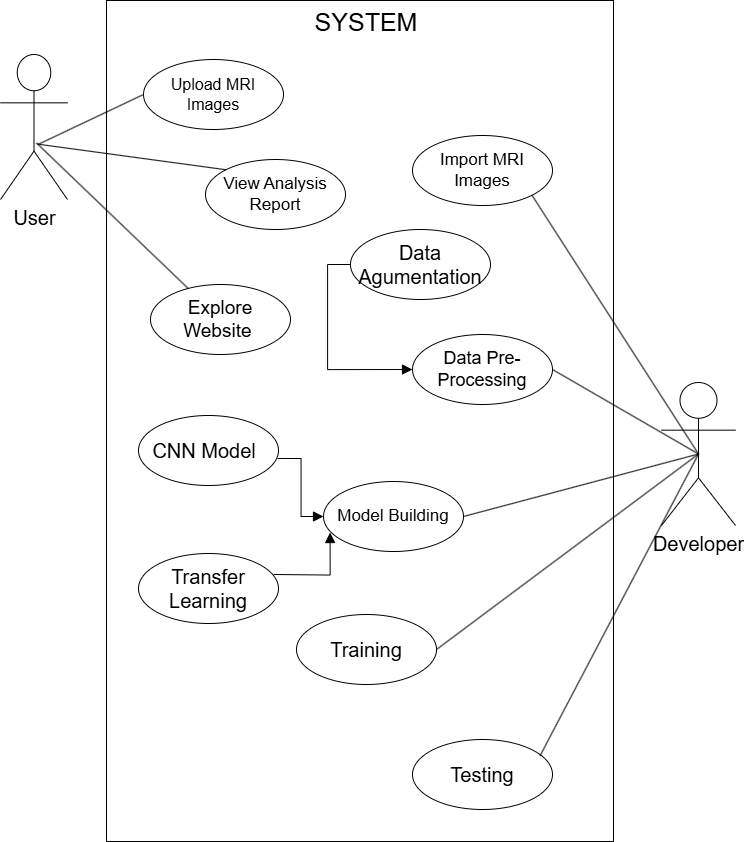
\includegraphics[width=0.85\linewidth]{Images/use.png}
    \caption{Use Case Diagram}
    \label{fig:Use Case Diagram}
\end{figure}
\subsubsection{Description of Algorithms}

\textbf{Convolutional Neural Network (\gls{cnn})}

A \gls{cnn} is a type of artificial neural network specifically designed for processing and classifying visual data. In this project, we developed a custom \gls{cnn} architecture tailored for medical imaging.

The model begins with an input layer that accepts brain \gls{mri} images resized to $150 \times 150$ pixels with three color channels. This is followed by a series of convolutional layers using \gls{relu} activation functions, each paired with MaxPooling layers to progressively reduce spatial dimensions and extract hierarchical features.

After the convolutional blocks, a flattening layer converts the extracted feature maps into a one-dimensional vector, which is then passed through fully connected Dense layers. Dropout regularization is employed to minimize overfitting. The final classification is done using a softmax output layer, enabling the model to distinguish between tumor and non-tumor cases.

The model is compiled using the Adam optimizer, categorical cross-entropy as the loss function, and accuracy as the evaluation metric. Data augmentation techniques such as random rotations, zooming, and flips are applied to improve the model's robustness and generalizability.

\begin{figure}[H]
    \centering
    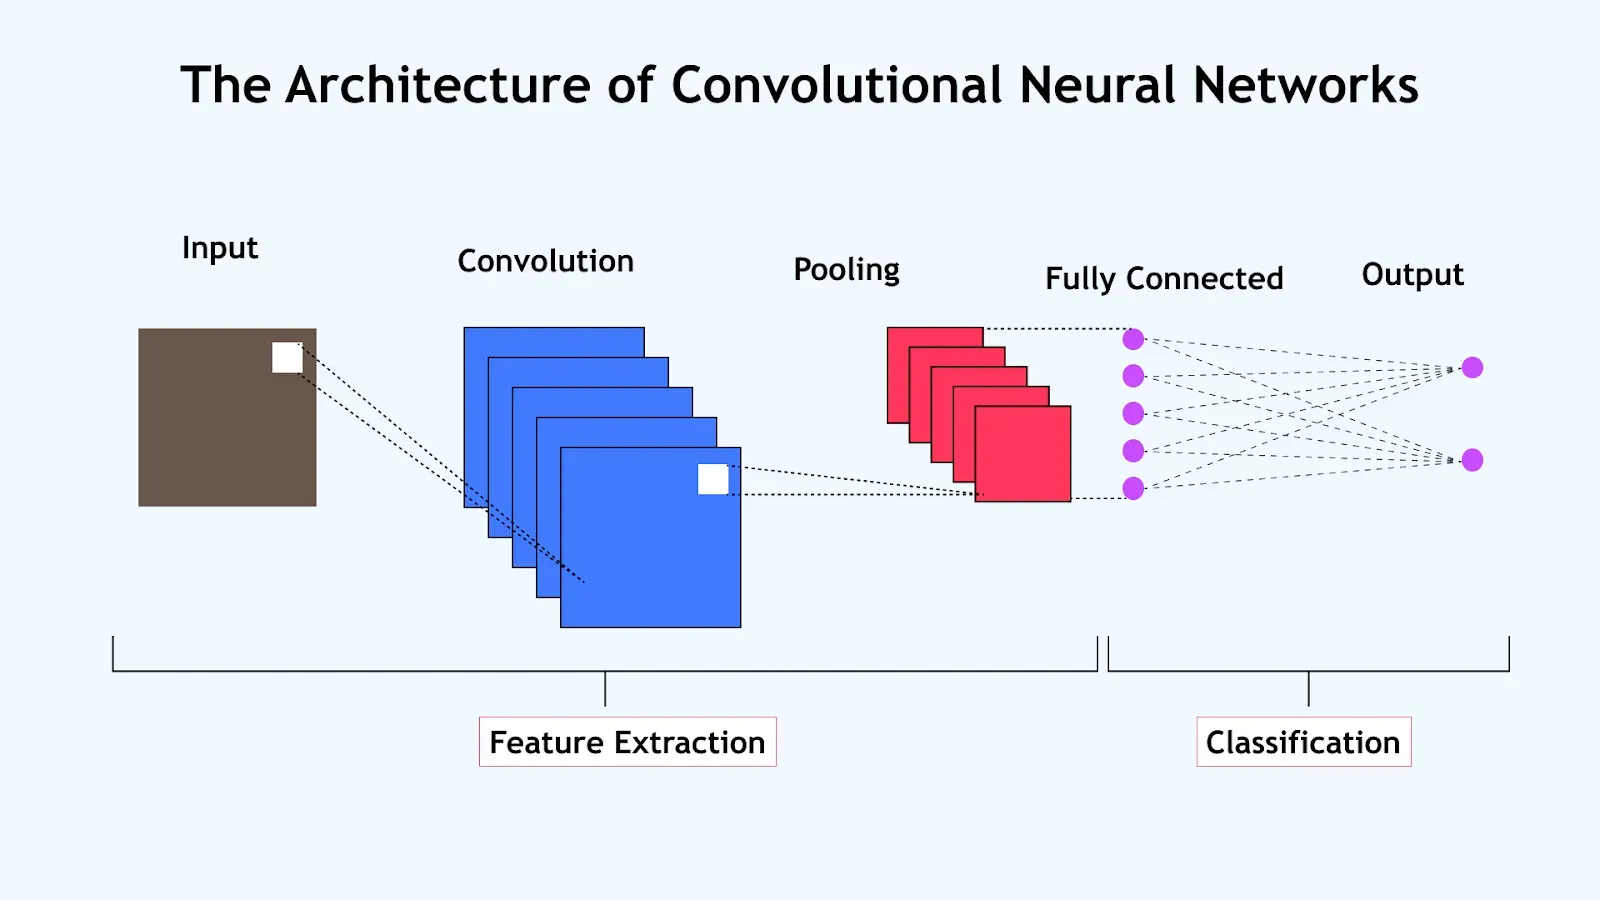
\includegraphics[width=0.85\linewidth]{Images/cnn.png}
    \caption{CNN Architecture}
    \label{fig:CNN Architecture}
\end{figure}

\textbf{Transfer Learning with \gls{vgg16}}

To complement the custom \gls{cnn} and further enhance accuracy, we integrate a transfer learning approach using the \gls{vgg16} architecture pretrained on the ImageNet dataset. \gls{vgg16} is a well-established deep network known for its simplicity and performance in image classification tasks.

In our approach, the \gls{vgg16} base model is used without its top classification layers. All convolutional layers of \gls{vgg16} are frozen to retain the pretrained features, which are known to capture generic visual patterns that are also relevant to medical images.

On top of the \gls{vgg16} base, we add a Global Average Pooling layer followed by fully connected Dense layers with \gls{relu} activations and Dropout. The final classification layer uses softmax activation to output probabilities for each class. This hybrid model combines the general visual understanding of \gls{vgg16} with task-specific learning layers adapted to brain tumor detection.

\begin{figure}[H]
    \centering
    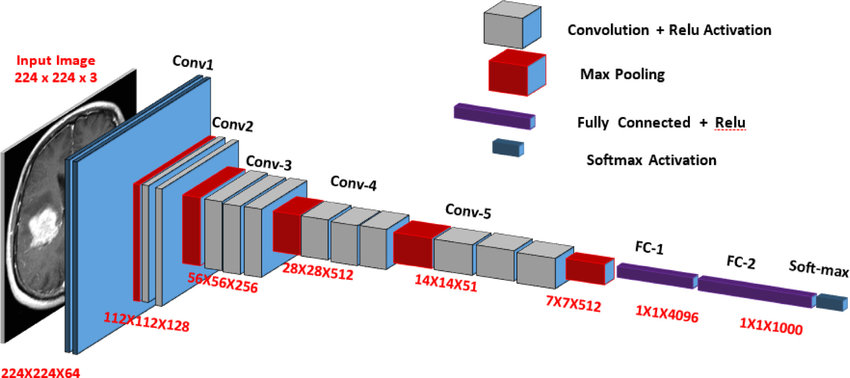
\includegraphics[width=0.85\linewidth]{Images/vgg16.jpg}
    \caption{VGG16 Architecture}
    \label{fig:VGG16 Architecture}
\end{figure}



